
%(BEGIN_QUESTION)
% Copyright 2006, Tony R. Kuphaldt, released under the Creative Commons Attribution License (v 1.0)
% This means you may do almost anything with this work of mine, so long as you give me proper credit

En lagertank med svært korrosiv væske får nivået målt med et \textit{bobbler}-system, der en transmitter måler mottrykket av luft inne i et ``dip tube'' som er ført ned i tanken:

$$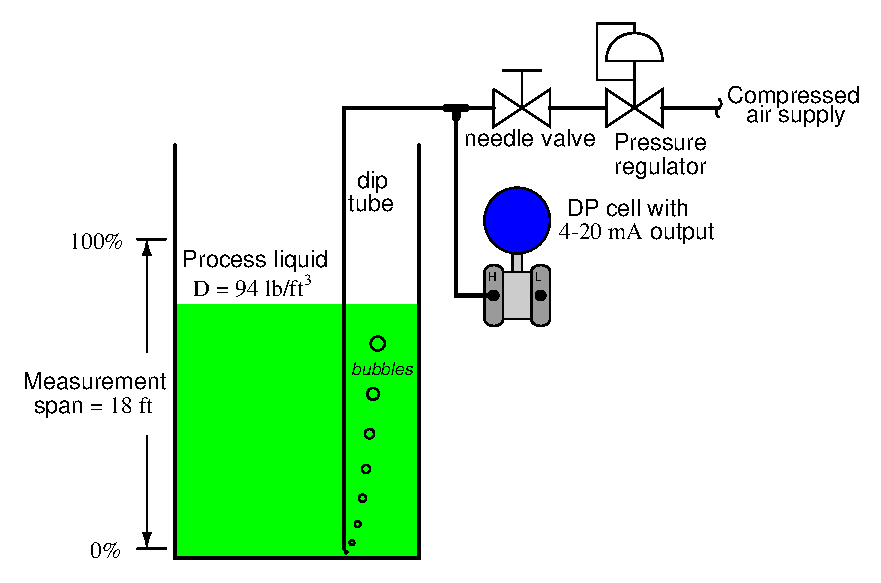
\includegraphics[width=12.5cm]{i00249x01.eps}$$

Forklar hvordan dette nivåmålesystemet virker, og hvordan det beskytter DP-cellen mot korrosiv påvirkning fra prosessvæsken.

\vskip 10pt

Fyll også ut en kalibreringstabell for differansetrykktransmitteren i dette nivåmålescenariet, med kalibreringstoleranse $\pm$ 0.5\%.  Anta at nedre måleverdi i prosessen (0\% nivå) er i nøyaktig samme høyde som bunnen av dypperøret:

% No blank lines allowed between lines of an \halign structure!
% I use comments (%) instead, so that TeX doesn't choke.

$$\vbox{\offinterlineskip
\halign{\strut
\vrule \quad\hfil # \ \hfil & 
\vrule \quad\hfil # \ \hfil & 
\vrule \quad\hfil # \ \hfil & 
\vrule \quad\hfil # \ \hfil & 
\vrule \quad\hfil # \ \hfil & 
\vrule \quad\hfil # \ \hfil \vrule \cr
\noalign{\hrule}
%
% First row
Prosess- & Prosent av & $\Delta$ trykk & Utgangssignal & Utgangssignal & Utgangssignal \cr
%
% Another row
nivå (m) & spenn (\%) & (cm W.C) & ideelt (mA) & min. (mA) & maks. (mA) \cr
%
\noalign{\hrule}
%
% Another row
  & 0 &  &  &  &  \cr
%
\noalign{\hrule}
%
% Another row
  & 10 &  &  &  &  \cr
%
\noalign{\hrule}
%
% Another row
  & 25 &  &  &  &  \cr
%
\noalign{\hrule}
%
% Another row
  & 50 &  &  &  &  \cr
%
\noalign{\hrule}
%
% Another row
  & 75 &  &  &  &  \cr
%
\noalign{\hrule}
%
% Another row
  & 90 &  &  &  &  \cr
%
\noalign{\hrule}
%
% Another row
  & 100 &  &  &  &  \cr
%
\noalign{\hrule}
} % End of \halign 
}$$ % End of \vbox

\underbar{file i00249}
%(END_QUESTION)





%(BEGIN_ANSWER)

\noindent
{\bf Delvis svar:}

% No blank lines allowed between lines of an \halign structure!
% I use comments (%) instead, so that TeX doesn't choke.

$$\vbox{\offinterlineskip
\halign{\strut
\vrule \quad\hfil # \ \hfil & 
\vrule \quad\hfil # \ \hfil & 
\vrule \quad\hfil # \ \hfil & 
\vrule \quad\hfil # \ \hfil & 
\vrule \quad\hfil # \ \hfil & 
\vrule \quad\hfil # \ \hfil \vrule \cr
\noalign{\hrule}
%
% First row
Prosess- & Prosent av & $\Delta$ trykk & Utgangssignal & Utgangssignal & Utgangssignal \cr
%
% Another row
nivå (m) & spenn (\%) & (cm W.C) & ideelt (mA) & min. (mA) & maks. (mA) \cr
%
\noalign{\hrule}
%
% Another row
0  & 0 &  &  &  &  \cr
%
\noalign{\hrule}
%
% Another row
  & 10 &  &  &  &  \cr
%
\noalign{\hrule}
%
% Another row
  & 25 & 206.53 & 8 &  &  \cr
%
\noalign{\hrule}
%
% Another row
  & 50 &  &  &  & 12.08 \cr
%
\noalign{\hrule}
%
% Another row
  & 75 &  &  &  &  \cr
%
\noalign{\hrule}
%
% Another row
  & 90 &  &  & 18.32 &  \cr
%
\noalign{\hrule}
%
% Another row
5.486 & 100 & 826.11 &  &  &  \cr
%
\noalign{\hrule}
} % End of \halign 
}$$ % End of \vbox

%(END_ANSWER)





%(BEGIN_NOTES)

Boblerør-prinsippet fungerer ved at et lite, kontinuerlig luftslipp presses ut i bunnen av dypperøret.  For å få luftbobler ut av røret må lufttrykket i røret minst være likt hydrostatisk trykk på væskesiden ved rørenden.  Dette mottrykket måles av transmitteren og er direkte proporsjonalt med væskenivå.

Siden kun luft i impulslinjen står i kontakt med transmitteren, og ikke selve prosessvæsken, blir transmitteren isolert fra den korrosive væsken.

\vskip 10pt

% No blank lines allowed between lines of an \halign structure!
% I use comments (%) instead, so that TeX doesn't choke.

$$\vbox{\offinterlineskip
\halign{\strut
\vrule \quad\hfil # \ \hfil & 
\vrule \quad\hfil # \ \hfil & 
\vrule \quad\hfil # \ \hfil & 
\vrule \quad\hfil # \ \hfil & 
\vrule \quad\hfil # \ \hfil & 
\vrule \quad\hfil # \ \hfil \vrule \cr
\noalign{\hrule}
%
% First row
Prosess- & Prosent av & $\Delta$ trykk & Utgangssignal & Utgangssignal & Utgangssignal \cr
%
% Another row
nivå (m) & spenn (\%) & (cm W.C) & ideelt (mA) & min. (mA) & maks. (mA) \cr
%
\noalign{\hrule}
%
% Another row
0 & 0 & 0 & 4 & 3.92 & 4.08 \cr
%
\noalign{\hrule}
%
% Another row
0.549 & 10 & 82.60 & 5.6 & 5.52 & 5.68 \cr
%
\noalign{\hrule}
%
% Another row
1.372 & 25 & 206.53 & 8 & 7.92 & 8.08 \cr
%
\noalign{\hrule}
%
% Another row
2.743 & 50 & 413.05 & 12 & 11.92 & 12.08 \cr
%
\noalign{\hrule}
%
% Another row
4.115 & 75 & 619.58 & 16 & 15.92 & 16.08 \cr
%
\noalign{\hrule}
%
% Another row
4.938 & 90 & 743.48 & 18.4 & 18.32 & 18.48 \cr
%
\noalign{\hrule}
%
% Another row
5.486 & 100 & 826.11 & 20 & 19.92 & 20.08 \cr
%
\noalign{\hrule}
} % End of \halign 
}$$ % End of \vbox

%INDEX% Calibration: table, level transmitter
%INDEX% Measurement, level: bubble tube (bubbler)
%INDEX% Measurement, level: calibration table
%INDEX% Measurement, level: dip tube
%INDEX% Measurement, level: hydrostatic pressure

%(END_NOTES)
